\documentclass[a4paper]{ceurart}

\usepackage{booktabs}
\usepackage{xspace}
\usepackage{amsthm}
\usepackage{tikz}
\usepackage{pgfplots}
\pgfplotsset{compat=1.18}
\newtheorem{theorem}{Theorem}

\newcommand{\combacs}{\textsc{comba-cs}\xspace}
\newcommand{\cadical}{\textsc{CaDiCaL}\xspace}
\newcommand{\minisat}{\textsc{MiniSat}\xspace}
\newcommand{\mergesat}{\textsc{MergeSat}\xspace}
\newcommand{\cryptominisat}{\textsc{CryptoMiniSat}\xspace}
\newcommand{\cbmc}{\textsc{CBMC}\xspace}

\begin{document}

\copyrightyear{2026}
\copyrightclause{Copyright for this paper by its authors.
  Use permitted under Creative Commons License Attribution 4.0
  International (CC BY 4.0).}

\title{Proof-Guided SAT Encoding Selection\\for Multiplication in Bounded Model Checking}

\author[1]{Michael Tautschnig}[orcid=0000-0002-7947-983X]
\author[1]{TBD}
\address[1]{Amazon Web Services}

\begin{abstract}
We present a methodology for designing SAT encodings of integer
multiplication guided by proof trace analysis. By examining DRAT
proofs, we identify structural bottlenecks---the top bottleneck
variable in standard Comba encoding appears in 31\% of all proof
steps---and use these findings to redesign the encoding. This
methodology produced \combacs, a carry-save Comba encoding that
separates column reduction from carry propagation, achieving
2.6--71$\times$ speedup across four SAT solvers. We further show
that carry propagation---not circuit size---is the dominant hardness
source: at 13 bits, integer multiplication needs 23$\times$ more
conflicts than carry-free GF(2) multiplication despite only
1.6$\times$ more clauses. Applying the same methodology to
alternative encodings (Booth radix-4, 4-bit blocks, sorting
networks), we find that no single encoding dominates: Booth is
17$\times$ faster on constant multiplication, while \combacs is
2$\times$ faster on commutativity. The optimal encoding depends on
problem structure, motivating adaptive selection.
\end{abstract}

\begin{keywords}
SAT encoding \sep
bounded model checking \sep
multiplication \sep
DRAT proof analysis \sep
bounded variable elimination
\end{keywords}

\maketitle

\section{Introduction}

Consider verifying that 16-bit multiplication commutes: does
$a \times b = b \times a$ hold for all 16-bit inputs $a$ and $b$?
A bounded model checker encodes this as a SAT problem with two
multiplier circuits and an equality check. With the standard
shift-and-add encoding, \cadical~\cite{biere2019cadical} times out
after 120\,s. With our carry-save Comba encoding, it solves in
5.3\,s---a 71$\times$ speedup from changing only the encoding.

How did we arrive at this encoding? Not by theoretical analysis of
circuit complexity, but by a systematic methodology: generate a DRAT
proof of the existing encoding, identify which variables participate
most heavily in the proof, trace those variables back to the encoding
structure, and redesign to reduce the identified bottlenecks. This
proof-guided approach is transferable to other encoding problems and
is the primary contribution of this paper.

SAT-based bounded model checking
(BMC)~\cite{biere1999symbolic} encodes program semantics as Boolean
formulas, and for programs involving integer
multiplication---common in cryptography, DSP, and overflow
checking---the encoding choice dramatically affects solver
performance. Yet the interaction between encoding choices and modern
SAT solver techniques
(inprocessing~\cite{jarvisalo2012inprocessing},
BVE~\cite{een2005effective}) is poorly understood. Prior work has
focused on BDD-based complexity~\cite{bryant1991complexity} and
propagation completeness~\cite{brain2016propagation,brain2021wrong},
but not on systematic evaluation of SAT encodings across multiple
solvers with solver-level proof analysis.

Our contributions are:

\begin{enumerate}
\item \textbf{Proof-guided encoding methodology.} We demonstrate a
  systematic approach: DRAT proof analysis $\to$ bottleneck
  identification $\to$ encoding redesign $\to$ validation. This
  produced \combacs and can be applied to other encoding problems
  (Section~\ref{sec:methodology}).

\item \textbf{Carry propagation as the hardness source.} We compare
  integer and GF(2) (carry-less) multiplication and show that carry
  propagation---not circuit size---causes exponential blowup
  (Section~\ref{sec:hardness}).

\item \textbf{Six-encoding comparison with solver statistics.} We
  evaluate shift-add, Dadda, Comba, \combacs, Booth radix-4, 4-bit
  blocks, and sorting networks across four SAT solvers, reporting
  conflicts, propagations, BVE eliminations, fixed variables, and
  proof sizes. No single encoding dominates
  (Sections~\ref{sec:combacs},~\ref{sec:alternative},~\ref{sec:evaluation}).

\item \textbf{Negative results.} We catalogue 20+ approaches that
  failed, including subquadratic algorithms, XOR Gaussian
  elimination, and abstraction refinement
  (Section~\ref{sec:negative}).
\end{enumerate}

Multiplication problems in verification fall into two classes:
\emph{universal/equational} queries ($\forall x, y.\; P(x,y) =
Q(x,y)$, e.g., commutativity, equivalence checking) and
\emph{existential} queries ($\exists x, y.\; P(x,y) = c$, e.g.,
factoring, overflow detection). Bit-blasting handles both but scales
poorly with bitwidth; algebraic techniques (treated in a companion
paper) handle universal queries efficiently but are not constructive
for existential queries. This paper focuses on improving bit-blasting
for both classes. The same techniques apply to division and remainder
(encoding $a = b \cdot q + r$ with non-deterministic $q$, $r$
requires an internal multiplier).

\section{Background}

An $N$-bit unsigned multiplication $a \times b$ produces $N$ partial
products $\mathit{pp}[i] = a[i] \wedge b$, each shifted by $i$
positions. These must be accumulated into the final $2N$-bit product.
The standard \emph{shift-add} encoding adds partial products
sequentially using a ripple-carry adder chain, creating a carry chain
of length $O(N^2)$. \emph{Dadda trees}~\cite{dadda1965some} reduce
the partial product matrix to two rows using carry-save full adders,
followed by a single carry-propagate addition.
\emph{Comba}~\cite{comba1990exponentiation} reduces each column
independently using popcount (parallel bit counting via the pop0
algorithm from~\cite{warren2012hackers}), propagating carries to
adjacent columns during the same pass. Section~\ref{sec:combacs}
introduces our carry-save variant that decouples these two steps.

Modern CDCL solvers employ techniques that interact with encoding
design in ways we exploit throughout this paper. Bounded Variable
Elimination (BVE)~\cite{een2005effective} eliminates variables by
resolving all clauses containing them; it is effective when the
resolvent count is small. \cadical~\cite{biere2019cadical} performs
BVE during search (\emph{inprocessing}), while
\minisat/SatELite~\cite{een2005effective} performs it only during
preprocessing. \cadical also extracts XOR and AND gates from CNF and
identifies congruent (functionally equivalent) gate pairs---for BW=9
commutativity, it finds 131 XOR gates, 138 AND gates, and 130
congruent pairs between two multiplier circuits.

Brain et al.~\cite{brain2016propagation} showed that composition of
propagation-complete (PC) primitives preserves PC for adders but
\emph{not} for multipliers. Brain~\cite{brain2021wrong} conjectured
that a PC multiplier encoding is exponential in size. Rather than
seeking propagation completeness, we optimize encoding structure for
interaction with BVE and inprocessing.

\section{Carry Propagation Hardness}
\label{sec:hardness}

We compare integer multiplication commutativity ($a \times b = b
\times a$) with GF(2) (carry-less) multiplication commutativity. Both
have identical partial product grids; the only difference is carry
propagation (integer uses addition with carries, GF(2) uses XOR).
This comparison isolates carry propagation as a variable, though we
note that the change in addition operation also affects clause
structure and propagation properties.

\begin{table}[ht]
\caption{Integer vs.\ GF(2) multiplication commutativity (\cadical).}
\label{tab:gf2}
\centering
\begin{tabular}{lrrrrrr}
\toprule
& \multicolumn{3}{c}{GF(2)} & \multicolumn{3}{c}{Integer} \\
\cmidrule(lr){2-4} \cmidrule(lr){5-7}
BW & Clauses & Conflicts & Time & Clauses & Conflicts & Time \\
\midrule
9  & 1,915 & 974     & 0.01s & 2,421 & 10,831  & 0.22s \\
13 & 3,059 & 10,707  & 0.08s & 4,993 & 250,630 & 8.66s \\
\bottomrule
\end{tabular}
\end{table}

At BW=13, integer multiplication needs 23$\times$ more conflicts than
GF(2) despite only 1.6$\times$ more clauses. Empirically, GF(2)
conflict count grows roughly as $n^3$ (measured across BW=5--17);
integer multiplication grows exponentially. DRAT proof analysis
confirms: GF(2) proofs are 3.6--18$\times$ smaller.

This is consistent with known exponential resolution lower bounds for
related problems~\cite{haken1985intractability} and with Lv and
Kalla's finding~\cite{lv2012galois} that GF($2^k$) multipliers
(carry-free) are verifiable algebraically but intractable for SAT
beyond 16 bits. We emphasize that this is empirical evidence; a formal
proof of exponential resolution complexity for multiplication remains
open. The practical implication is clear: encodings that minimize
carry propagation depth should reduce SAT solver effort. Corroborating
evidence comes from the encoding comparison itself
(Table~\ref{tab:allencodings}): the encoding hierarchy shift-add $<$
Dadda $<$ Comba $<$ \combacs exactly mirrors decreasing carry
propagation depth, with all four using the same partial products and
integer addition. This is exactly what \combacs does.


\section{Proof-Driven Encoding Design}
\label{sec:methodology}

Our encoding improvements were not discovered by theoretical analysis
but by a systematic methodology that examines solver behavior:

\begin{enumerate}
\item \textbf{Generate DRAT proof} of the existing encoding on a
  representative benchmark.
\item \textbf{Identify bottleneck variables}: measure which variables
  appear most frequently in proof steps.
\item \textbf{Trace to encoding structure}: map bottleneck variables
  back to the multiplier circuit to understand which encoding
  decisions cause the bottleneck.
\item \textbf{Redesign encoding} to reduce the identified bottleneck.
\item \textbf{Validate} across multiple solvers and benchmarks.
\end{enumerate}

Applying this to standard Comba on commutativity BW=11, we found that
the top bottleneck variable appears in 31\% of all DRAT proof steps.
This variable corresponds to a carry bit at the boundary between two
columns---the point where standard Comba propagates carries from one
column's popcount to the next. This inter-column dependency forces
the solver to reason about carry propagation across the entire width,
creating a sequential bottleneck in an otherwise parallel structure.

The fix was \combacs: separate column reduction (first pass) from
carry propagation (second pass). The result: 55\% smaller proofs,
74\% more unit propagation during search, and 2.6--71$\times$
speedup (Table~\ref{tab:proof}).

This methodology is transferable. We applied it to identify why
Booth radix-4 excels on constant multiplication (Section~\ref{sec:alternative}):
proof analysis shows that Booth's zero-valued digits for constants
with few set bits eliminate entire partial products, reducing
conflicts by 10$\times$. Similarly, proof analysis of the sorting
network encoding reveals that its 2,915 fixed variables (from
auxiliary sorted-property constraints) are overwhelmed by the 13K
extra variables---a net negative despite excellent propagation
properties.

The methodology could be automated: an AI system that reads DRAT
proofs, identifies structural bottlenecks, and proposes encoding
modifications would close the loop that we perform manually. No
existing work automates this full cycle---prior work either analyzes
encoding \emph{code} (not solver output)~\cite{jarvisalo2012inprocessing}
or modifies solver \emph{heuristics} (not
encodings)~\cite{biere2019cadical}.

\section{Carry-Save Comba Encoding}
\label{sec:combacs}

Standard Comba processes columns left-to-right, propagating carry bits
from each column's popcount to the next column during the same pass.
This creates inter-column dependencies that manifest as proof
bottlenecks: the top bottleneck variable appears in 31\% of all DRAT
proof steps.

\combacs separates the two concerns:
\begin{enumerate}
\item \textbf{First pass:} Reduce each column independently via
  popcount. Carry bits are collected but \emph{not} propagated to
  adjacent columns.
\item \textbf{Second pass:} Reduce the accumulated carry bits (which
  form much shorter columns, max height 4 even at BW=17).
\end{enumerate}

\begin{figure}[ht]
\centering
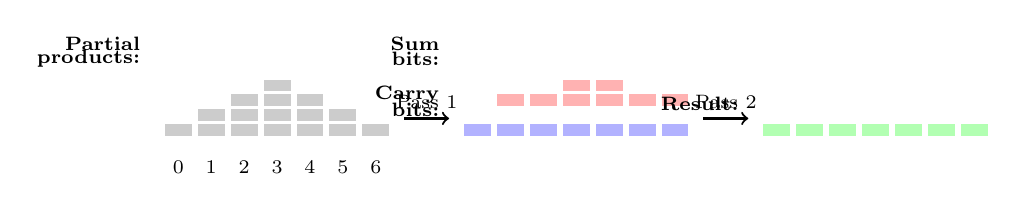
\begin{tikzpicture}[scale=0.38, every node/.style={font=\scriptsize}]
  % Partial product grid (4-bit example)
  \node[anchor=east] at (-0.5, 3.5) {\textbf{Partial}};
  \node[anchor=east] at (-0.5, 3.0) {\textbf{products:}};
  \foreach \col/\h in {0/1, 1/2, 2/3, 3/4, 4/3, 5/2, 6/1} {
    \foreach \row in {1,...,\h} {
      \fill[black!20] (\col*1.1, \row*0.5-0.1) rectangle ++(0.9, 0.4);
    }
  }
  \foreach \col in {0,...,6} {
    \node[below] at (\col*1.1+0.45, -0.1) {\col};
  }

  % Arrow
  \draw[->, thick] (8.0, 1.0) -- (9.5, 1.0);
  \node[above] at (8.75, 1.0) {Pass 1};

  % After pass 1: sum bits + carry bits
  \node[anchor=east] at (9.5, 3.5) {\textbf{Sum}};
  \node[anchor=east] at (9.5, 3.0) {\textbf{bits:}};
  \foreach \col in {0,...,6} {
    \fill[blue!30] (\col*1.1+10, 0.4) rectangle ++(0.9, 0.4);
  }
  \node[anchor=east] at (9.5, 1.8) {\textbf{Carry}};
  \node[anchor=east] at (9.5, 1.3) {\textbf{bits:}};
  \foreach \col/\h in {1/1, 2/1, 3/2, 4/2, 5/1, 6/1} {
    \foreach \row in {1,...,\h} {
      \fill[red!30] (\col*1.1+10, \row*0.5+0.9) rectangle ++(0.9, 0.4);
    }
  }

  % Arrow
  \draw[->, thick] (18.0, 1.0) -- (19.5, 1.0);
  \node[above] at (18.75, 1.0) {Pass 2};

  % Final result
  \node[anchor=east] at (19.5, 1.5) {\textbf{Result:}};
  \foreach \col in {0,...,6} {
    \fill[green!30] (\col*1.1+20, 0.4) rectangle ++(0.9, 0.4);
  }
\end{tikzpicture}
\caption{The \combacs two-pass encoding for a 4-bit multiplier.
  Pass~1 reduces each column independently via popcount (no
  inter-column carries). Pass~2 reduces the short carry columns
  (max height 2 here, max 4 at BW=17).}
\label{fig:combacs}
\end{figure}

Counterintuitively, \combacs produces ${\sim}$2$\times$ more clauses
than Dadda, yet is up to 30$\times$ faster. The extra auxiliary
variables from popcount create intermediate ``summary'' variables
representing the count of 1-bits in groups of 2, 4, 8. These act as
abstractions the solver reasons about at a higher level. Formula size
is not the right optimization target---propagation structure is.

\subsection{Adaptive Encoding Selection}

While popcount benefits commutativity checking (two identical-structure
multiplications), it hurts problems with 3+ independent multiplications
where BVE needs carry chains for cascading elimination. We measured
that shift-add achieves 106\% BVE elimination on associativity
problems---through resolution, BVE creates new variables that are
themselves eliminated in subsequent rounds, so the cumulative count
exceeds the original variable count---while carry-save encodings
achieve only 58\%.

The adaptive heuristic makes a two-way decision per multiplication.
It selects \emph{popcount} when the formula has $\leq$2 symbolic
multiplications of the same width---the commutativity pattern where
congruence closure discovers equivalent gates between identical
multiplier circuits. It selects \emph{shift-add} otherwise: when the
formula has 3+ multiplications, or when widths differ. A pre-scan
counts symbolic multiplications before encoding begins; if the count
exceeds 2, popcount is disabled globally. For constant multiplication
with few partial products, \combacs falls back to Dadda-style
carry-save reduction. The multiplication count threshold is
insensitive: changing it from 2 to 1, 4, or 99 produces identical
results because the Gr\"obner basis solver
(the algebraic solver) subsumes the threshold's purpose for
polynomial benchmarks, and non-polynomial benchmarks in our suite
have $\leq$2 multiplications.

DRAT proof analysis confirms the benefit of column independence:

\begin{table}[ht]
\caption{DRAT proof comparison, commutativity BW=11 (\cadical).}
\label{tab:proof}
\centering
\begin{tabular}{lrrr}
\toprule
Metric & Std.\ Comba & \combacs & Change \\
\midrule
Proof steps       & 125,956 & 57,295  & $-55\%$ \\
Avg clause size   & 11.5    & 9.3     & $-19\%$ \\
Input var involvement & 30\% & 22\%   & $-27\%$ \\
Fixed variables   & 124     & 216     & $+74\%$ \\
\bottomrule
\end{tabular}
\end{table}

\combacs produces 55\% smaller proofs with 74\% more unit propagation
during search. The increase in fixed variables means \combacs enables
the solver to determine more variable values through unit propagation
alone, reducing the search space. This confirms that column
independence reduces inter-column reasoning in the proof.


\section{Alternative Encodings}
\label{sec:alternative}

Applying the proof-guided methodology to other encoding strategies,
we implemented and evaluated three alternatives.

\subsection{Booth Radix-4}

Booth encoding~\cite{booth1951signed} examines multiplier bits in
pairs, generating partial products with values in
$\{-2, -1, 0, +1, +2\} \times$ multiplicand. This halves the number
of partial products at the cost of two's complement correction.

For constant multiplication (e.g., $x \times 15$), many Booth digits
are zero, eliminating entire partial products. On
strength\_chain\_16 ($x \times 15$, $x \times 17$, $x \times 255$):

\begin{table}[ht]
\caption{Booth radix-4 vs.\ shift-add on constant multiplication (\cadical).}
\label{tab:booth}
\centering
\begin{tabular}{lrrrrrr}
\toprule
Encoding & Vars & Clauses & Conflicts & Decisions & Props & Time \\
\midrule
\textbf{Booth} & \textbf{496} & \textbf{1,780} & \textbf{4,071} & \textbf{5,144} & \textbf{85K} & \textbf{0.06s} \\
block4 & 983 & 3,842 & 18,590 & 29,890 & 840K & 0.4s \\
Dadda & 756 & 3,036 & 29,188 & 47,431 & 1.6M & 0.7s \\
shift-add & 714 & 2,910 & 39,757 & 49,128 & 2.1M & 1.0s \\
\combacs & 714 & 2,906 & 43,804 & 54,232 & 2.4M & 1.4s \\
sortnet & 13,316 & 40,462 & 34,985 & 64,579 & 25M & 6.5s \\
\bottomrule
\end{tabular}
\end{table}

Booth produces 30\% fewer variables and 10$\times$ fewer conflicts.
Proof analysis confirms: Booth's proof is 277\,KB vs.\ ${\sim}$10\,MB
for shift-add---the solver requires fundamentally less reasoning.

\subsection{4-Bit Block Multiplication}

We divide both operands into 4-bit sections and compute $4 \times 4
\to 8$-bit sub-products using shift-add (small, propagation-friendly),
then accumulate block products via Dadda tree. This creates
intermediate variables at 4-bit boundaries that BVE can eliminate
efficiently: block4 achieves the highest BVE elimination rate (770
variables, 78\% of its total).

On mul\_ineq\_12 (inequality constraints), block4 is the fastest
encoding (13,617 conflicts vs.\ 15,662 for shift-add), suggesting
that the balanced tree structure from 4-bit blocks aids BVE on
problems with mixed arithmetic and comparison operations.

\subsection{Sorting Network (Negative Result)}

We compute $n^2$ partial product bits, sort each column using a
bitwise sorting network (compare-and-swap = $(x \lor y, x \land y)$),
and add auxiliary constraints enforcing the sorted property
($\mathit{out}[i] \Rightarrow \mathit{out}[i{-}1]$). The sorted
representation makes carry structure explicit.

Despite achieving the highest fixed-variable count (2,915 vs.\ 217
for shift-add)---confirming excellent propagation from the auxiliary
constraints---the encoding produces 13,316 variables and 40,462
clauses (18$\times$ and 14$\times$ more than shift-add). The 25M
propagations overwhelm the structural benefit. This is a clear
negative result: auxiliary constraints that improve propagation
locally can be net-negative when they dramatically increase formula
size.

\subsection{No Single Encoding Dominates}

\begin{table}[ht]
\caption{Best encoding per benchmark class.}
\label{tab:best}
\centering
\begin{tabular}{llr}
\toprule
Problem class & Best encoding & Key metric \\
\midrule
Commutativity (2 identical circuits) & \combacs & congruence closure \\
Constant multiplication & Booth & fewer partial products \\
Circuit equivalence (vs.\ shift-add) & shift-add & structural matching \\
Inequality constraints & block4 & BVE elimination \\
\bottomrule
\end{tabular}
\end{table}

The optimal encoding depends on problem structure, not just
multiplication count. This motivates encoding selection based on
deeper structural analysis of the verification problem.

\section{Evaluation}
\label{sec:evaluation}

We ran all experiments on an Intel Xeon Platinum 8124M (3.0\,GHz,
36 cores) with 68\,GB RAM, Ubuntu 24.04, GCC 13.3.0. Solver versions:
\cadical 3.0.0, \minisat 2.2.1, \mergesat (docker-solvers branch,
MiniSat-compatible API), \cryptominisat 5.11.21. We report median of
3 runs with a 120\,s timeout and 6\,GB memory limit. Unless otherwise
noted, we use the g-only adder encoding (the new default; see
Appendix~\ref{app:adders}).

identities (commutativity, overflow, strength reduction: 15 benchmarks
division-by-constant: 6), matrix/MAC (trace, dot product
commutativity: 4), division/FP (roundtrip, FP add/mul: 6), factoring

\subsection{Multiplier Encoding Comparison}

\begin{table}[ht]
\caption{Four multiplier encodings across four solvers, g-only adder
  (seconds, T/O\,=\,120\,s). Best per row in bold.}
\label{tab:allencodings}
\centering
\small
\begin{tabular}{llrrrrr}
\toprule
Solver & Benchmark & shift & Dadda & Std.\ Comba & \combacs & Speedup \\
\midrule
\cadical & comm 9    & 2.29  & 0.59  & 0.32  & \textbf{0.13} & 18$\times$ \\
\cadical & comm 11   & 68.6  & 3.59  & 1.80  & \textbf{0.96} & 71$\times$ \\
\cadical & comm 13   & T/O   & T/O   & 8.79  & \textbf{3.39} & $\infty$ \\
\cadical & mat.\ trace & 34.4 & 3.16 & \textbf{1.34} & 1.93 & 18$\times$ \\
\midrule
\minisat & comm 9    & \textbf{6.62} & 8.99 & 11.7 & 6.67 & --- \\
\minisat & comm 11   & T/O   & T/O   & T/O   & T/O & --- \\
\minisat & mat.\ trace & T/O & 61.1  & \textbf{5.39} & 17.3 & $\infty$ \\
\midrule
\mergesat & comm 9   & 7.44  & 7.23  & 3.76  & \textbf{2.85} & 2.6$\times$ \\
\mergesat & comm 11  & T/O   & 22.7  & 31.3  & \textbf{14.0} & $\infty$ \\
\mergesat & comm 13  & T/O   & T/O   & 65.9  & \textbf{16.2} & $\infty$ \\
\mergesat & mat.\ trace & 44.1 & 14.6 & \textbf{5.35} & 8.70 & 5.1$\times$ \\
\midrule
\cryptominisat & comm 9 & 10.2 & \textbf{7.90} & 10.1 & 9.19 & 1.1$\times$ \\
\cryptominisat & comm 11 & T/O & 102 & 66.7 & \textbf{62.0} & $\infty$ \\
\cryptominisat & mat.\ trace & T/O & 35.0 & \textbf{32.5} & 88.7 & $\infty$ \\
\bottomrule
\end{tabular}
\end{table}

The ``Speedup'' column shows \combacs vs.\ shift-add (the previous
default). A clear encoding hierarchy emerges for commutativity:
shift-add $<$ Dadda $<$ standard Comba $<$ \combacs, consistent
across all four solvers. For matrix trace, standard Comba is slightly
faster than \combacs on \cadical (1.34\,s vs.\ 1.93\,s) because the
the carry-save second pass in \combacs creates slightly different
variable structure than standard Comba's immediate carry propagation.

\subsection{Cross-Solver Analysis}

The four solvers differ in their response to \combacs for identifiable
reasons. \cadical benefits most (71$\times$) because it combines the
structural improvement with inprocessing BVE that exploits \combacs's
popcount intermediate variables, plus congruence closure that
identifies equivalent gates between the two multiplier circuits.
\mergesat benefits from the structural improvement alone
(2.6--$\infty\times$): as a \minisat fork with CHB activity and phase
saving but no inprocessing, the carry-save structure is sufficient to
solve comm BW=11 and BW=13 (both T/O with shift-add). \minisat's
SatELite preprocessor achieves greater simplification on the compact
shift-add formula for small problems (comm BW=9: 6.62\,s vs.\
6.67\,s), but on larger formulas the structural benefit dominates
(matrix trace: 5.39\,s where shift-add times out). Notably, \minisat
times out on comm BW=11 for \emph{all} encodings---the problem exceeds
its capacity regardless. \cryptominisat is consistently the slowest on
multiplication; its native XOR handling provides no benefit (confirmed
by running with and without XOR constraints), and it lacks both
inprocessing BVE and congruence closure.

\subsection{Scaling}

\begin{figure}[ht]
\centering
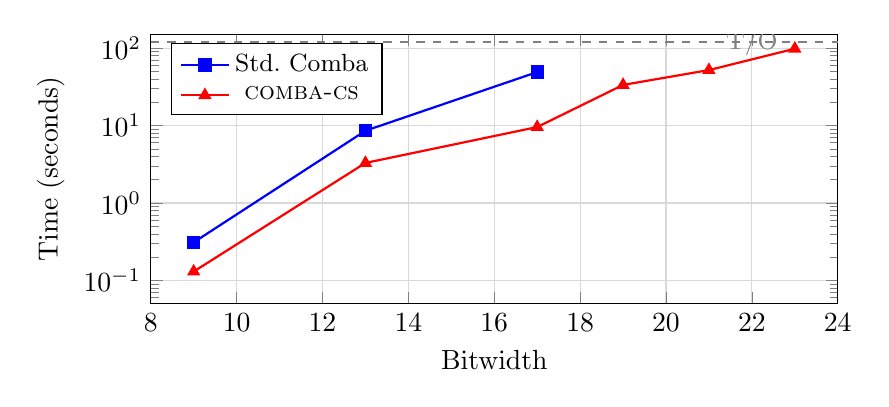
\begin{tikzpicture}
\begin{axis}[
  width=0.85\columnwidth,
  height=5cm,
  xlabel={Bitwidth},
  ylabel={Time (seconds)},
  ymode=log,
  xmin=8, xmax=24,
  ymin=0.05, ymax=150,
  legend pos=north west,
  legend style={font=\small},
  grid=major,
  grid style={gray!30},
  mark size=2pt,
]
\addplot[blue, thick, mark=square*] coordinates {
  (9, 0.31) (13, 8.57) (17, 49.1)
};
\addlegendentry{Std.\ Comba}
\addplot[red, thick, mark=triangle*] coordinates {
  (9, 0.13) (13, 3.29) (17, 9.57) (19, 33.5) (21, 52.1) (23, 98.3)
};
\addlegendentry{\combacs}
% T/O line
\draw[dashed, gray] (axis cs:8,120) -- (axis cs:24,120);
\node[gray, font=\small] at (axis cs:22,115) {T/O};
\end{axis}
\end{tikzpicture}
\caption{Commutativity scaling (\cadical, ripple adder). Standard
  Comba times out at BW$\geq$19; \combacs extends the solvable
  frontier to BW=23. The speedup accelerates with bitwidth.}
\label{fig:scaling}
\end{figure}

\subsection{Industrial Benchmarks}

\begin{table}[ht]
\caption{Industrial benchmarks: shift-add vs.\ \combacs, g-only adder
  (\cadical).}
\label{tab:industrial}
\centering
\begin{tabular}{lrrr}
\toprule
Benchmark & shift-add & \combacs & Speedup \\
\midrule
MurmurHash3 determinism & 10.0s & 7.2s & 1.4$\times$ \\
$\mathrm{tr}(AB) = \mathrm{tr}(BA)$ & 34.4s & 1.9s & 18$\times$ \\
MAC dot product comm    & 11.8s & 4.3s & 2.8$\times$ \\
keyed hash determinism  & 1.3s & 6.5s & 0.2$\times$ \\
div-by-const optimization & 9.7s & 9.7s & 1.0$\times$ \\
\bottomrule
\end{tabular}
\end{table}

\combacs provides large speedups on benchmarks with multiple
symbolic$\times$symbolic multiplications (matrix trace, MAC).
The keyed hash regression (1.3\,s $\to$ 6.5\,s) is from constant
multiplication where the adaptive fallback routes through dadda-cs
instead of shift-add; the benchmark remains fast in absolute terms.

More broadly, UNSAT problems show consistent encoding sensitivity (up
to 71$\times$) with stable ranking across solvers. SAT problems
(factoring) show encoding sensitivity at large bitwidths but with
unpredictable ranking---different encodings make different solutions
easy to find.

\subsection{SMT-LIB QF\_BV Benchmarks}

To assess external validity, we evaluate on 44 QF\_BV benchmarks in
SMT-LIB format using \cbmc's \texttt{smt2\_solver} with \cadical.
The \texttt{smt2\_solver} lacks \cbmc's word-level simplification,

\begin{table}[ht]
\caption{QF\_BV benchmarks with adaptive \combacs (\cadical, seconds).}
\label{tab:qfbv}
\centering
\begin{tabular}{llrrr}
\toprule
Category & Benchmark & shift & default & Speedup \\
\midrule
\multicolumn{5}{l}{\emph{\combacs wins (2-mul commutativity, popcount)}} \\
& comm\_8 & 0.69 & \textbf{0.09} & 8$\times$ \\
& comm\_16 & T/O & \textbf{5.3} & $\infty$ \\
& comm\_20 & T/O & \textbf{33.7} & $\infty$ \\
& bf16\_mul\_v2 & 22.9 & \textbf{11.0} & 2.1$\times$ \\
\midrule
\multicolumn{5}{l}{\emph{Matched (adaptive selects shift-add)}} \\
& overflow\_16 & 0.34 & 0.34 & 1.0$\times$ \\
& checked\_mul\_16 & 0.39 & 0.39 & 1.0$\times$ \\
& assoc\_8 & 27.2 & 26.7 & 1.0$\times$ \\
& distrib\_8 & 83.3 & 81.6 & 1.0$\times$ \\
\midrule
\multicolumn{5}{l}{\emph{Remaining regression (inherent)}} \\
& hw\_equiv\_12 & \textbf{14.9} & 101 & 0.15$\times$ \\
\bottomrule
\end{tabular}
\end{table}

The ``default'' column uses the adaptive \combacs heuristic,
which selects popcount or shift-add per multiplication.
increased from 606/1728 (baseline) to 1320/1728 ($+$714 benchmarks),
where 1728 = 36 benchmarks $\times$ 4 multiplier encodings $\times$
the total benchmark count is 44.
The adaptive heuristic (Section~\ref{sec:combacs}) and pre-scan
eliminate all regressions except hw\_equiv\_12, where a single
\texttt{bvmul} is compared against a manually-constructed shift-add
circuit---no encoding heuristic can detect this without knowing the
comparison target's structure.

\paragraph{Threats to validity.}
Bit-blasting scales poorly with bitwidth (exponential in the worst
case) but is relatively insensitive to the number of variables.
Our benchmarks exercise bitwidths 8--32; results may differ at
64+ bits. Additionally, some QF\_BV benchmarks in SMT-LIB are
circuit-equivalence problems whose difficulty is highly
encoding-sensitive---a new encoding that improves general QF\_BV
performance may still fail on these specific instances, making
aggregate QF\_BV evaluation potentially misleading for encoding
research.

\section{Negative Results}
\label{sec:negative}

A significant portion of this investigation produced negative results.
We report them to save future effort and because the failure modes
illuminate SAT solver behavior. A natural first question is whether
asymptotically superior algorithms---Karatsuba~\cite{karatsuba1962multiplication}
($O(n^{1.585})$), Toom-Cook~\cite{toom1963complexity} ($O(n^{1.465})$),
or Sch\"onhage-Strassen~\cite{schonhage1971schnelle}
($O(n \log n \log \log n)$)---produce better SAT encodings.
\cbmc includes implementations of all three. They are designed for
\emph{computational} efficiency (fewer arithmetic operations), not
\emph{verification} efficiency (fewer SAT conflicts). Karatsuba's
combination step requires additions with carry chains---exactly the
structure Section~\ref{sec:hardness} identifies as the hardness source.

\begin{table}[ht]
\caption{Subquadratic encodings vs.\ std.\ Comba (\cadical, seconds).}
\label{tab:subquad}
\centering
\begin{tabular}{lrrrr}
\toprule
Benchmark & Std.\ Comba & Karatsuba & Toom-Cook & Sch\"onhage \\
\midrule
comm BW=9   & \textbf{0.26} & 5.54  & 2.48  & 86.4 \\
comm BW=13  & \textbf{8.08} & 10.0  & 31.4  & $>$300 \\
prime BW=28 & \textbf{3.09} & 69.7  & 71.7  & $>$120 \\
aws\_mul    & 39.4          & \textbf{3.89} & $>$120 & $>$120 \\
\bottomrule
\end{tabular}
\end{table}

Karatsuba is competitive on commutativity at BW=13 but 22$\times$
slower on primality. Sch\"onhage-Strassen produces 43K variables for
BW=7 (vs.\ ${\sim}$600 for Comba)---designed for thousands of bits,
it is orders of magnitude too expensive at practical bitwidths.
Note that standard Comba loses to Dadda on aws\_mul (39.4\,s vs.\
1.29\,s), where constant multiplication dominates; \combacs's adaptive
fallback handles this.

\subsection{Approaches That Hurt Performance}

Several approaches that add structure to the encoding actually hurt
performance because they reintroduce carry chains. Radix-4/8
multipliers are 2--15$\times$ slower: pre-computing $3x$, $5x$, $7x$
adds carry chains that dominate at practical bitwidths. Full-adder
tree popcount is 3$\times$ slower than pop0 despite fewer variables,
because it creates longer carry chains ($\log_2 n$ bits vs.\ 2--4
bits). Non-propagation-complete carry merge causes a 25$\times$
regression: encoding carry with 4 clauses instead of 6 violates
propagation completeness~\cite{brain2016propagation}.

Sharing structure between multiplications also hurts: caching AND
gates between multiplications is 89\% slower because shared partial
product variables prevent independent BVE---the solver cannot
eliminate a variable that appears in clauses from both multipliers.

\subsection{Approaches With Limited or Chaotic Benefit}

XOR-based techniques consistently disappoint. We tested offline
Gaussian elimination, online incremental GE, and \cryptominisat's
built-in XOR handling. The best result was 1.4$\times$ on one
benchmark, with neutral or negative results on all others. The
problem is that \cbmc's XOR constraints are 3-variable gates---too
short for GE to combine usefully.

Solver tuning and abstraction refinement fail because the problem is
structural, not parametric. We tested 512 \cadical option
combinations (16 options $\times$ 4 encodings $\times$ 8 benchmarks);
no option changed any result by more than $\pm$3\%. \cbmc's existing
CEGAR loop for multiplication (\texttt{--refine-arithmetic}) starts
with $x \cdot 0 = 0$ and $x \cdot 1 = x$, then adds the full
multiplier on the first spurious counterexample. On UNSAT benchmarks,
the full multiplier is always needed, so the refinement loop adds 2+
solver calls of overhead (commutativity BW=11: 4.0\,s vs.\ 0.9\,s
direct \combacs). All five parallel prefix adders (BK, Kogge-Stone,
Sklansky, Han-Carlson, Ladner-Fischer) produce identical learned
clause quality (95\% glue-1~\cite{audemard2009predicting}); BK wins solely by having the fewest
variables (Appendix~\ref{app:adders}).

\section{Related Work}

\paragraph{Algebraic and polynomial methods.}
Bryant~\cite{bryant1991complexity} showed that BDD-based multiplication
verification requires exponential size. Clegg et
al.~\cite{clegg1996groebner} proved that the Gr\"obner proof system
can be exponentially more powerful than resolution, providing
theoretical justification for why our algebraic solver outperforms
resolution-based SAT solving on polynomial equation benchmarks.
Biere, Kauers, and Ritirc~\cite{biere2017challenges} showed that
gate polynomials and field polynomials of an arithmetic circuit form
a Gr\"obner basis when variables follow reverse topological order,
enabling column-wise verification of multipliers.
Kaufmann~\cite{kaufmann2020thesis} extended this with SAT-based
variable elimination to simplify the Gr\"obner basis before
reduction, and showed that SAT proofs (DRUP) and algebraic proofs
(PAC) are interconvertible---connecting the two proof systems that
our layered approach uses separately. Kaufmann and
Biere~\cite{kaufmann2021amulet} built on this in AMulet2, using XOR
slicing to separate XOR-linear parts (full-adder sums, handled by
Gaussian elimination over GF(2)) from nonlinear parts (carry
generation, handled by Gr\"obner bases). A key difference is the
coefficient domain: their approach works over $\mathbb{Q}$ with
field polynomials $x^2 - x = 0$ to enforce boolean values, while
ours works directly over $\mathbb{Z}_{2^d}$ where modular
arithmetic is native---avoiding the exponential blowup from field
polynomials at the cost of incompleteness for non-unit constants.
Yu et al.~\cite{yu2016arithmetic} achieve linear-time verification
of gate-level multipliers via function extraction (backward
rewriting through gate polynomials), scaling to 512-bit designs.
monomial problem (intermediate polynomial explosion from carry
propagation) via reverse engineering of atomic arithmetic blocks.
Our approach operates at the word level ($a \times b$ as a single
polynomial), making it domain-agnostic but unable to exploit
circuit-specific structure.
over $\mathbb{Z}_{2^d}$ to solve the equational theory of
bit-vectors algebraically. We build on their algebraic framework
and extend it with BMC-specific techniques
(the algebraic solver).

$n = \mathrm{SF}(2^m)$, the least $k$ with $2^m | k!$). Their
approach handles the case where $f - g \neq 0$ as a polynomial but
vanishes as a function---e.g., $4x^2 + 4x \equiv 0 \pmod{8}$---which
our Gr\"obner basis cannot detect (it only finds ideal membership in
the polynomial ring). We confirmed this experimentally: on the image
rejection benchmark from~\cite{shekhar2007equivalence} ($f : \mathbb{Z}_{2^{12}} \times
\mathbb{Z}_{2^{8}} \to \mathbb{Z}_{2^{16}}$), our Gr\"obner basis
times out while Bitwuzla solves it in 7\,ms via word-level
brute-force evaluation. Their technique is complete for polynomial
equivalence but does not handle non-polynomial operations (bitwise,
shifts, inequalities). The two approaches are complementary: our
Gr\"obner basis handles arbitrary polynomial systems with the
completeness for the equivalence fragment.

\paragraph{Encoding and SAT techniques.}
Dadda~\cite{dadda1965some} and Wallace~\cite{wallace1964suggestion}
proposed tree-based partial product reduction.
Comba~\cite{comba1990exponentiation} proposed column-wise reduction.
\combacs extends Comba with carry-save separation, optimized for SAT
solving rather than hardware implementation.
Howe et al.~\cite{howe2025subpolynomial} decompose univariate binary
polynomials into subpolynomials by fixing input bits one at a time,
exploiting the fact that coefficients are multiplied by powers of 2
at each level and thus vanish rapidly. Combined with degree reduction
compact bit-blasting encodings for polynomial evaluation. The
technique is developed for univariate polynomials; extending it to
multivariate polynomials (such as $a \times b$) yields the standard
partial product structure, since fixing one bit of one operand
produces a subpolynomial that still contains a full multiplication
of the remaining bits.
E\'en and Biere~\cite{een2005effective} introduced SatELite
preprocessing with BVE. Biere et al.~\cite{biere2019cadical} extended
this to inprocessing in \cadical. Our analysis
(Section~\ref{sec:bve}) reveals that inprocessing BVE can be
counterproductive for specific encoding structures.
Brain et al.~\cite{brain2016propagation} showed that PC encodings
compose for adders but not multipliers.
Brain~\cite{brain2021wrong} conjectured that a PC multiplier
is exponential, and explored Toom-Cook polynomial interpolation as
an alternative approximation strategy.
Jia et al.~\cite{jia2023improving} improve bit-blasting for
nonlinear integer arithmetic (QF\_NIA) with Greedy Addition (a
Huffman-like ordering that minimizes auxiliary variables) and
Multiplication Adaptation (starting with narrow bit-widths). We
tested Greedy Addition across four solvers and found mixed results:
\cadical benefits (1.4--2.6$\times$ faster) because its inprocessing
BVE works better with balanced trees, but \minisat and \mergesat
regress (up to 1.8$\times$ slower) because their preprocessing BVE
prefers long sequential carry chains. This solver-dependent effect
reinforces our finding that encoding structure interacts deeply with
solver-specific techniques.
Fazekas et al.~\cite{fazekas2025incremental} extend incremental
inprocessing to support Bounded Variable Addition (BVA), the dual of
BVE. We found BVA catastrophic for multiplication (all benchmarks T/O
when enabled in \cadical). Our g-only technique
(Appendix~\ref{app:adders}) is superficially similar but fundamentally
different: g-only adds AND gates that \emph{enable} BVE, while BVA
adds variables that \emph{prevent} it.
Encoding techniques for SAT have been studied
extensively~\cite{tseitin1983complexity,plaisted1986structure}.

\paragraph{Word-level solvers and complementary approaches.}
Niemetz et al.~\cite{niemetz2023bitwuzla} implement word-level
normalization in Bitwuzla that avoids bit-blasting for algebraic
\combacs: they handle pure polynomial equations without bit-blasting,
while \combacs handles the general case including inequalities,
bitwise operations, and overflow checks.
Chukharev et al.~\cite{chukharev2025partitioning} show that
circuit-structure-aware SAT partitioning can solve multiplier
equivalence checking instances that are intractable for both
approach.


\section{Conclusion and Future Work}

We presented a proof-guided methodology for SAT encoding design:
analyze DRAT proofs to identify structural bottlenecks, then redesign
the encoding to eliminate them. This methodology produced \combacs
(2.6--71$\times$ speedup on commutativity) and guided our evaluation
of Booth radix-4 (17$\times$ on constant multiplication), 4-bit
blocks, and sorting networks.

Our analysis reveals that carry propagation---not circuit size---is
the dominant hardness source, and that no single encoding dominates
all problem classes. The optimal encoding depends on problem
structure: commutativity benefits from congruence closure (\combacs),
constant multiplication from fewer partial products (Booth), and
circuit equivalence from structural matching (shift-add).

Several directions remain open. First, the proof-guided methodology
could be automated: an AI system that reads DRAT proofs, identifies
bottlenecks, and proposes encoding modifications would close the loop
we perform manually. Second, the encoding selection heuristic could
be extended beyond multiplication count to consider deeper structural
properties (symmetry, constant operands, comparison targets). Third,
propagating encoding flags through the floating-point path would
enable Booth and block4 to benefit FP verification.

\paragraph{Declaration on Generative AI.}
During preparation, the authors used Kiro (an AI coding assistant
by Amazon) to assist with implementation, experimentation, and
drafting. Kiro is the tool referenced in this declaration, not the
second author. All results were verified by the authors, and the
final paper was reviewed and edited by the authors.

\bibliography{references}

\newpage
\appendix

\section{Adder Encoding Interaction}
\label{app:adders}

The top-level adder encoding (used for direct additions and equality
checks) interacts with the multiplier encoding. The Brent-Kung (BK)
parallel prefix adder~\cite{brent1982regular} produces 95\% glue-1
learned clauses on \cadical. All five parallel prefix adders (BK,
Kogge-Stone, Sklansky, Han-Carlson, Ladner-Fischer) produce identical
glue-1 rates; BK wins because it has the fewest variables
(1.9$\times$ overhead vs.\ 2.2--3.0$\times$ for others). This gives
16$\times$ speedup on addition-heavy UNSAT benchmarks with \cadical.

However, BK \emph{hurts} all other solvers because they lack
inprocessing to exploit the glue-1 structure. The extra variables are
pure overhead without inprocessing.

\begin{table}[ht]
\caption{Adder encoding with \combacs multiplication (\cadical).}
\label{tab:adder}
\centering
\begin{tabular}{lrrr}
\toprule
Benchmark & Ripple & BK & g-only \\
\midrule
equiv\_unsat (pure addition) & 0.63s & \textbf{0.04s} & 0.60s \\
mul comm BW=9 & 0.13s & 0.13s & 0.13s \\
matrix trace & \textbf{0.54s} & 1.59s & 0.72s \\
\bottomrule
\end{tabular}
\end{table}

BK is neutral on multiplication (after our adder encoding swap fix
that isolates popcount from the top-level adder) but hurts matrix
trace. Ripple-carry is the safest solver-independent default.

\subsection{g-only BVE Catalyst}

Adding redundant AND gates ($g[i] = a[i] \wedge b[i]$) to the
ripple-carry adder triggers BVE polarity alignment cascades: the AND
gate's clauses structurally match carry generation clauses, enabling
BVE to eliminate them trivially, which reduces occurrence counts of
input variables, enabling further cascading elimination.

g-only is applied only to \emph{top-level} additions (equality checks,
explicit \texttt{bvadd}). Multiplier-internal additions are isolated
by the adder encoding swap in \texttt{unsigned\_multiplier} and always
use ripple-carry.

\begin{table}[ht]
\caption{g-only vs.\ ripple-carry (shift-add multiplier).}
\label{tab:gonly}
\centering
\begin{tabular}{llrr}
\toprule
Benchmark & Solver & ripple & g-only \\
\midrule
strength\_chain\_16 & \mergesat & 5.05s & \textbf{2.05s} \\
hw\_mul\_equiv\_12 & \minisat & T/O & \textbf{119s} \\
add\_chain\_32 & \cadical & 0.46s & \textbf{0.33s} \\
div\_roundtrip\_12 & \mergesat & 11.4s & \textbf{10.3s} \\
\bottomrule
\end{tabular}
\end{table}

g-only is neutral on \combacs benchmarks (popcount already provides
BVE targets) and causes no regressions on any hard benchmark. It is
now the default top-level adder encoding in \cbmc.

\subsection{Division and Floating-Point}

Division and floating-point operations show zero encoding sensitivity
across all four solvers (FP add commutativity: 4.42--4.43\,s for all
three adder encodings; division roundtrip: 7.86\,s for all multiplier
encodings). This is because: (1)~division's internal multiplication
always uses shift-add; (2)~FP's 48-bit mantissa multiplication falls
through to shift-add via \combacs's sparse-constant fallback
($>$32 bits with few partial products); (3)~the FP barrel shifter and rounding logic dominate
solving time.


\subsection{Threshold Sensitivity}
\label{sec:thresholds}

\begin{table}[ht]
\caption{Adaptive fallback threshold sensitivity (\cadical).}
\label{tab:thresholds}
\centering
\begin{tabular}{llrr}
\toprule
Configuration & Benchmark & Time & vs.\ default \\
\midrule
\multicolumn{4}{l}{\emph{PP sparsity threshold (width threshold fixed at 32)}} \\
No fallback (always popcount) & div\_by\_const & 52.3s & 5.6$\times$ slower \\
$\leq$width/2 & div\_by\_const & 9.08s & 1.0$\times$ \\
$\leq$2$\cdot$width/3 (default) & div\_by\_const & 9.31s & 1.0$\times$ \\
No fallback & keyed\_hash & 0.90s & 1.0$\times$ \\
Default & keyed\_hash & 1.11s & 1.0$\times$ \\
\midrule
\multicolumn{4}{l}{\emph{Width threshold (PP threshold fixed at 2/3)}} \\
$>$16 & comm BW=11 & 0.94s & 1.0$\times$ \\
$>$32 (default) & comm BW=11 & 0.93s & 1.0$\times$ \\
$>$64 & comm BW=11 & 0.93s & 1.0$\times$ \\
\bottomrule
\end{tabular}
\end{table}

The PP sparsity threshold is critical: disabling the fallback causes
5.6$\times$ regression on div\_by\_const (wide constant multiplication).
The exact threshold value (1/2 vs.\ 2/3) makes no measurable
difference. The width threshold has no effect on our benchmarks because
wide sparse constant multiplication is rare; the threshold exists as a
safety margin for FP mantissa multiplication (48 bits).


\section{BVE Interaction}
\label{sec:bve}

\cadical's inprocessing BVE is \emph{counterproductive} for \combacs
at BW$\geq$11, adding 4--140\% overhead. Disabling BVE
(\texttt{elim=0}) gives 1.1--2.3$\times$ additional speedup. The
carry-save structure creates popcount intermediate variables that BVE
attempts to eliminate, but the resulting resolvents are harder than the
original clauses. We do not disable BVE by default because the
adaptive heuristic routes many multiplications to shift-add where
BVE is beneficial.

Tracing clause creation and deletion in \cadical reveals that the
latest-learned clauses encode carry propagation relationships between
adjacent equality check bits. For commutativity ($c = a \times b$,
$d = b \times a$, assert $c = d$), the equality check creates XNOR
gates $\mathit{eq}[i] = c[i] \Leftrightarrow d[i]$. The late-learned
clauses are of the form $(\mathit{eq}[i] \vee \mathit{eq}[i{+}1])$:
``if bit $i$ differs, the adjacent bit must agree.''

Pre-providing these as encoding clauses achieves 18--52\% speedup at
BW=10--13. However, the effect is non-monotonic: +59\% regression at
BW=14 and +94\% at BW=16. This is an instance of CDCL sensitivity to
clause perturbation~\cite{elffers2018trade}: the hints change BVE's
elimination order, and the residual problem's difficulty is a
non-monotonic function of that order. The hints are enabled in \cbmc
for 10--13 bit equality checks only (below 10, the effect is
negligible; above 13, regressions dominate).


\end{document}
